% Phylofriend User Guide
%
% For PDF output: pdflatex phylofriend.tex
% For HTML output: plastex pyhlofriend.tex
%
% For Graphics:
% Use PNG format to avoid problems with HTML conversion.
% Recommended size: < 13cm x 18cm (width x height).
% Recommended resolution: 300 dpi.
%
% Use fixed width instead of textwidth, so that plastex can
% recognize the graphics size. For example use
% 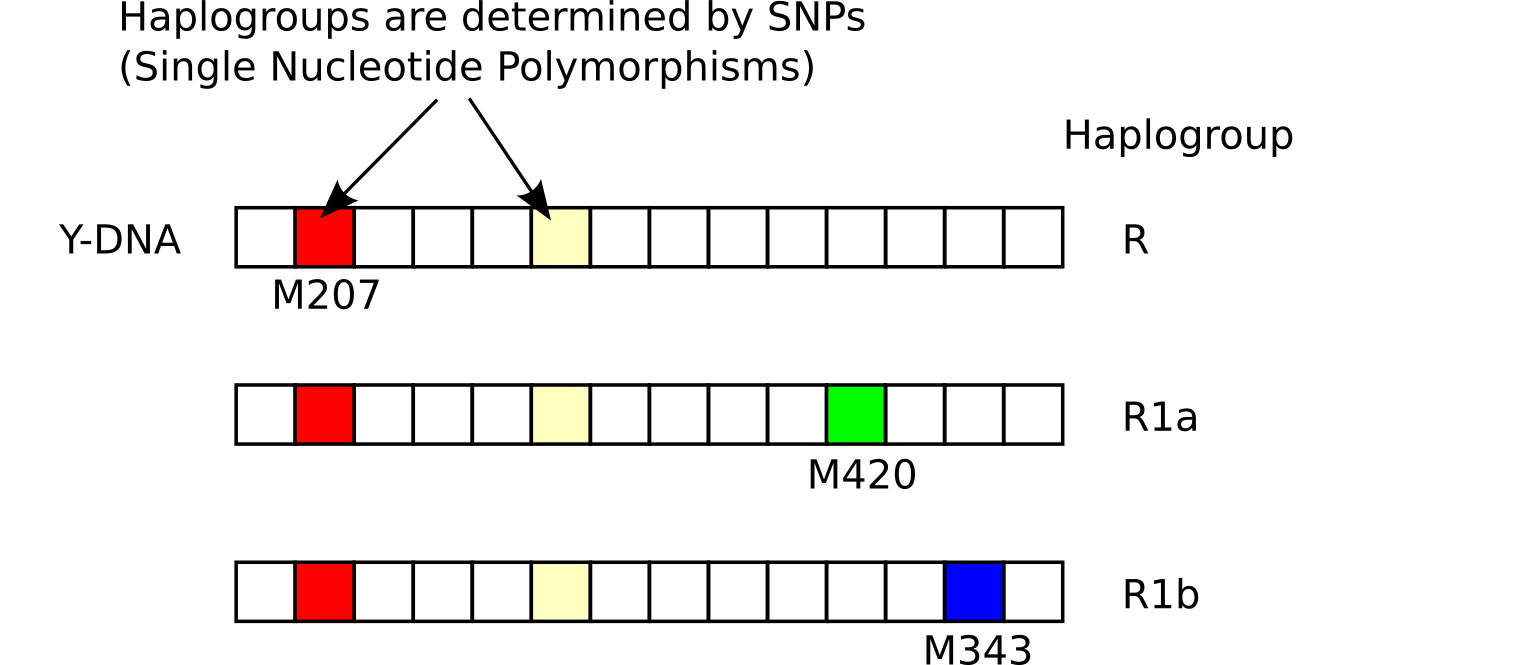
\includegraphics[width=13cm]{img/haplogroups.png}
% instead of
% 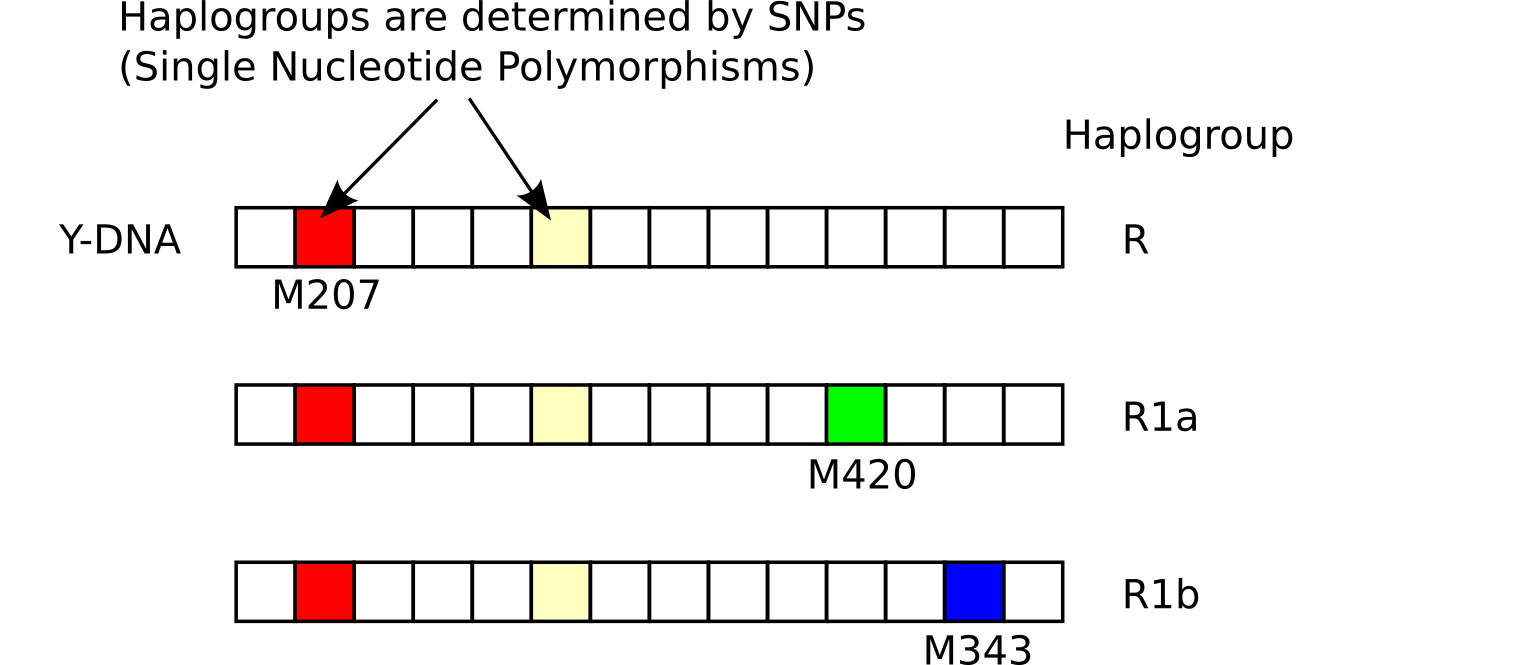
\includegraphics[width=\textwidth]{img/haplogroups.png}


\documentclass[12pt,a4paper]{article}
\usepackage[utf8]{inputenc}
\usepackage[english]{babel}
\usepackage[colorlinks=true, urlcolor=blue, linkcolor=blue]{hyperref}
\usepackage{graphicx}

\begin{document}
\begin{titlepage}

\title{Phylofriend User Guide}

\author{Dirk Struve\\
phylofriend at projectory.de\\
\href{https://github.com/yogischogi/phylofriend/}{https://github.com/yogischogi/phylofriend/}}
\date{\today}
\end{titlepage}
\maketitle

\tableofcontents
\section{Introduction}

Phylofriend's main purpose is to calculate genetic distances from
Y-DNA data. The results can be used as input for the
PHYLIP\cite{Phylip} program to create phylogenetic trees.

When I started creating phylogenetic trees I often found
myself in a difficult position. As a Linux user I was missing
some of the tools available under Windows. So I started
to write this program to fill in the gaps and make myself
comfortable again.

This does not mean that you can not use Phylofriend when
working under Windows or the Mac. But currently there is
no binary distribution available and you will probably face
a hard time installing Phylofriend and the associated programs.
So I only recommend this if you are an experienced user.

Phylofriend has some nice features. It can be used

\begin{itemize}
\item to create phylogenetic trees using the
	\href{http://evolution.genetics.washington.edu/phylip.html}{PHYLIP}\cite{Phylip}
	program. Y-STR values from Family Tree DNA projects can
	easily be imported.
\item as a programming library. Phylofriend is written in
	Google's \href{http://golang.org/}{Go} programming
	language. This language is not only suited to solve
	Google's large scale programming problems. It is also
	an excellent tool for part time programmers who have
	to concentrate on their projects (often students).
\item to extract Y-DNA data from Family Tree DNA projects
	and convert it into simpler text files that are
	better suited for further processing.
\item to automate phylogenetic tree creation. Phylofriend
	is a command line tool and this scares many people
	away. But if you have to repeat the same tasks over
	and over again you will eventually start to write some
	scripts and this is where command line tools come in
	handy.
\end{itemize}

I hope this program will be useful. Have a good time!

\vspace{1em} Dirk




\section{Installation}

This guide is mainly targeted towards persons who use Linux Mint
or other Linux versions of the Debian family. Some familiarity
with the use of Linux commands is assumed.

Currently there are no binary distributions available for
Windows or the Mac. Users of these operating systems can
use Phylofriend as well, but they will experience some
laborious installation work. The best way is to follow the
instructions provided on the
\href{http://golang.org/}{Go} home page and the
\href{http://evolution.genetics.washington.edu/phylip.html}{PHYLIP}
home page.

The following list applies to Linux users only:

\begin{enumerate}
\item Make sure that the Go programming language is installed.
	If not it can be installed by typing\\
	\texttt{sudo apt-get install golang}
\item Read the Go
	\href{http://golang.org/doc/install}{Getting Started}
	guide. Make sure to set your \emph{GOPATH} variable and
	include it in your \emph{PATH} so that Go programs can be
	found.
\item For the creation of phylogenetic trees install the
	PHYLIP program package by typing\\
	\texttt{sudo apt-get install phylip}
\item Fetch the Phylofriend program with\\
	\texttt{go get code.google.com/p/phylofriend}
\item Install the program with\\
	 \texttt{go install code.google.com/p/phylofriend}
\end{enumerate}


\section{Command Line Options}

Command line options may be given in arbitrary order.

\begin{description}
\item[-help] Prints available program options.
\item[-personsin] Filename or directory of files containing the
	persons' Y-STR values. If this is a single file it must contain
	results for multiple persons. The input file format is CSV
    (comma separated values) or text format.

	If a directory is provided for input it must contain multiple
	files in YFull format, each file containing the results for
	a single person. The person's ID is extracted from the filename.
\item[-labelcol] Number of the column that is used for labels
	when reading CSV files.
\item[-mrin] Filename of the mutation rates to use.
\item[-anonymize] If this is true persons' names are replaced by numbers.
\item[-modal] Creates modal haplotype and performs TMRCA calculation.
\item[-phylipout] Filename for the distance matrix that can be fed into
	the PHYLIP\cite{Phylip} program.
\item[-mrout] Filename for the output of the currently used mutation rates.
\item[-txtout] Filename for text output of persons and Y-STR values.
\item[-nmarkers] Uses only the given number of markers for calculations.
\item[-gentime] Generation time.
\item[-cal] Calibration factor.
\item[-reduce] Reduces the number of persons by the given factor
	 (for large numbers of samples).
\end{description}


\section{Examples}

\subsection{Create a Phylogenetic Tree}

\begin{enumerate}
\item Copy persons' data from a Family Tree DNA project website into
	a spreadsheet. If the Y-STR values do not appear properly try
	inserting them into the spreadsheet as unformatted text.
\item Save the spreadsheet in CSV (comma separated values)
	format, for example \emph{persons.csv}.
\item Start a terminal or command line interpreter and go
	to the directory where you stored \emph{persons.csv}.
\item Create a matrix of genetic distances by typing\\
	\texttt{phylofriend -personsin persons.csv -phylipout infile}
\item Use the PHYLIP program to create a tree in Newick format
	with\\
	\texttt{/usr/lib/phylip/bin/kitsch}\\
	You will need to answer some questions. Usually the
	default values are good enough. The results will be
	two text files, one named \emph{outtree} which contains
	the tree in Newick format and another one named
	\emph{outfile} which contains a more human readable
	description.
\item Create an image of the tree by typing\\
	\texttt{/usr/lib/phylip/bin/drawgram}\\
	Use \emph{outtree} as the input file name.
	The resulting tree will be stored in a file named 
	\emph{plotfile}.

	A nice alternative to visualize the tree is the use of the
	\href{http://www.trex.uqam.ca/index.php?action=newick&project=trex}
	{Trex}\cite{Trex}
	webserver. You can copy the contents of the file \emph{outtree}
	into the Trex window.
\end{enumerate}

If you do not specify a file containing mutation rates
Phylofriend will use average 37 marker values as default.
They can be found in \cite{Kly12}.


\subsection{Pimp Your Tree with Nicer Labels}

By default Phylofriend assumes that your persons input file's
first column contains a list of IDs. This is usually a Family
Tree DNA Kit number. The resulting tree is hard to read. Many
projects keep names in another column. You can access this 
column by using the \emph{labelcol} option. Suppose your second
column contains names. You can create a distance matrix with
names instead of IDs by typing

\noindent\texttt{phylofriend -personsin persons.csv -labelcol 2\\
-phylipout infile}

Due to compatibility issues with other programs the labels
must be 10 characters long and may only contain 8-bit
characters. Phylofriend will apply a transformation to
make sure that the requirements are fulfilled 
but the result is sometimes a bit strange.

You can also use the \emph{labelcol} option to create trees
that contain the origins of people or the haplogroups. Although
I strongly recommend to build trees only from people who
belong to the same haplogroup this is sometimes useful if
you want to know if different haplogroups are close on their
Y-STR values.

If you want to publish your tree you will often need to
protect the privacy of the members. This is what the
\emph{anonymize} option is for. By typing

\noindent\texttt{phylofriend -personsin persons.csv -phylipout infile -anonymize}

you will get a distance matrix where the names are replaced
by numbers.


\subsection{Use a Specific Set of Mutation Rates}

The first example uses Phylofriend's build in mutation rates
which are average values for the standard 37 marker test.
Phylofriend supports the use of arbitrary mutation rates by
the \emph{mrfile} option. The \emph{phylofriend/mutationrates}
directory contains some files with mutation rates. The average
mutation rates where taken from \cite{Kly12}.
If you like to compare on 67 markers you can use

\noindent\texttt{phylofriend -personsin persons.csv -phylipout infile\\
-mrin github.com/yogischogi/phylofriend/mutationrates/67-average.txt}


\subsection{Calibrate Your Data}

Mutation rates depend on the method applied to calculate
genetic distances and the sample populations used. Mutations
themselves occur by coincidence. Average mutation rates
often yield acceptable results but in most cases you will
have to calibrate your data especially if you want to
calculate in years.

Phylofriend provides two options for data calibration:
\emph{gentime}, the generation time in years and
\emph{cal} an additional calibration factor. Internally
they are just multiplied together but using two separate
factors seems more convenient for typical use cases.

The default value for the generation time is 25 years.
For time spans over the last few hundred years a generation
time of 30 years often yields better results. This can
be done by

\noindent\texttt{phylofriend -personsin persons.csv -phylipout infile\\
-gentime 30}

It is often difficult to calibrate data because you need a
reliable paper trail or a well defined historic event. If
you are lacking both you can try to apply Klyosov's statistical
method\cite{Kly09}. For large enough sample sizes this will
effectively reduce the statistical error but you will still
be left with an unknown systematical one.


\subsection{Count Mutations}

The \emph{phylofriend/mutationrates} directory contains
sets of mutation rates where all markers are set to 1.
This makes mutation counting easy but you will need an
additional little trick. Internally Phylofriend uses
average values. So it is possible to compare persons who
have tested on different sets of markers.

If you want to count mutations for example on a 37 marker
scale, you must multiply Phylofriend's internal results with
37. The easiest way to archive this is by misusing the
\emph{gentime} option. 

\noindent\texttt{phylofriend -personsin persons.csv\\
-mrin github.com/yogischogi/phylofriend/mutationrates/37-1.txt\\
-phylipout distancecount.txt -gentime 37}


\subsection{Extract Data from a Spreadsheet}

Spreadsheet data is often uncomfortable to handle, especially
if you want to write your own program and need to parse it.
For this purpose Phylofriend supplies the \emph{txtout}
option. It writes data to a text file in simplified form.

The easiest way to use it is

\noindent\texttt{phylofriend -personsin persons.csv -txtout persons.txt}

This extracts the data from \emph{persons.csv} and writes
it to \emph{persons.txt}. The first column of \emph{persons.txt}
contains the first column found in \emph{persons.csv}, usually
a set of IDs. The following columns contain the Y-STR values.
All columns are separated by tabs.

If you want to use another column you can use the
\emph{labelcol} option:

\noindent\texttt{phylofriend -personsin persons.csv -txtout persons.txt\\
-labelcol 2}

This extracts the second column from \emph{persons.csv} and
writes it to the first column of \emph{persons.txt}.

When using the \emph{txtout} option you will need to specify
how many Y-STR values are written to the text file. This is
done by \emph{nvalues}. Phylofriend will write the same number
of Y-STR values to each line. Missing values are written as
0, larger sets of Y-STR values are truncated. This is how to
write a full set of 111 markers:

\noindent\texttt{phylofriend -personsin persons.csv -txtout persons.txt\\
-nvalues 111}

















\section{Technicalities}

\subsection{Source Code Documentation}

To access the source code documentation point your
web browser to:

\begin{itemize}
\item \href{http://godoc.org/github.com/yogischogi/phylofriend}{http://godoc.org/github.com/yogischogi/phylofriend}
\end{itemize}

If you want to modify the source code it is best to
use \emph{godoc} locally on your computer.

\begin{enumerate}
\item If \emph{godoc} is not yet installed install it by typing\\
	\texttt{sudo apt-get install golang-go.tools}\\
	(Linux Mint)
\item Start the documentation web server with\\
	\texttt{godoc -http=:6060}
\item Point your web browser to \texttt{localhost:6060}.
\item Click on \emph{Packages} and search for \emph{phylofriend}.
\end{enumerate}

This will give you a nice overview of the internal program
documentation. You can also click on function names to browse
the source code.


\subsection{Mutation Model}

The two basic mutation models are the infinite alleles model
and the stepwise mutation model as explained by Bruce Walsh\cite{Wal02}.
Phylofriend uses a hybrid mutation model. Most markers are
calculated using the stepwise model, palindromic markers are
calculated as described in \cite{Can14}.

As the method for calculating the genetic distance is likely
to change with time please look at the internal program
documentation if you need more details.


\subsection{Mutation Rates}

The directory \emph{phylofriend/mutationrates} contains
files with predefined mutation rates.


\subsection*{Average Mutation Rates}

\begin{itemize}
\item 12-average.txt
\item 37-average.txt
\item 67-average.txt
\item 111-average.txt
\item 390-average.txt (experimental)
\item 500-average.txt (experimental)
\end{itemize}

In these files average mutation rates are used for the
corresponding set of markers. The mutation rates for 12,
37, 67 and 111 markers were taken from \cite{Kly12}.

The mutation rates for 390 and 500 markers are experimental.
They were derived by comparing YFull data of the
\href{http://yfull.com/groups/list/}{R1b-M343 (xP312 xU106) project}
to Family Tree DNA data from members of the
\href{https://www.familytreedna.com/groups/ht-3-5new/about/background}{R1b-M269 (P312- U106-) project}.
500-average.txt uses all known Y-STR markers that are
reported by YFull and Family Tree DNA. 390-average.txt leaves
out most of the palindromic markers. This marker set should
suffer less from saturation effects.

These mutation rates are useful for genealogical purposes.
During genealogical time frames (about 400 years) long time
stable markers rarely change. If such an event happens a
son may be immediately 1000 years away from his father in
terms of genetic distance. This is a correct result because
mutations are governed by coincidence and such events do
happen from time to time but it does not make much sense
to place a son far away from his family. So very stable
markers are purposely underweighted by using average
values.


\subsection*{12 Marker Single Mutation Rates}

\begin{itemize}
\item 12.txt
\item 37-12.txt
\item 67-12.txt
\item 111-12.txt
\end{itemize}

These files are basically the same as the average mutation
rates files but for the first 12 markers the mutation rates
are set per marker. This puts appropriate weight on
very stable markers. The mutation rates were taken from
Wikipedia\cite{Wiki-List_of_DYS_markers}. Although there
may be some doubt if data from Wikipedia can be trusted 
the first 12 markers are well known and they are in use
for a long time. So I just adopted them. The values should be
good enough for most purposes.

For each file the 12 marker mutation rates were multiplied
by a calibration factor so that their average value matches
that from the rest of the file.

These files are useful for deeper history or if you
observe changes on long time stable markers. If several
persons share the same value on a very stable marker they
probably belong together. So try these mutation rates to
see if the results make more sense than those obtained by
using average markers.


\subsection{CSV Input Format}

Example:

\begin{verbatim}
id1,"Dirk Struve",Germany,R1b-CTS4528,13,24,14,11,11-14,12,...
id2,"Pyl. O. Friend",Germany,R1b-CTS4528,13,24,14,11,11-14,...
\end{verbatim}

When importing a file in comma separated values format the
first column must contain IDs. An arbitrary number of columns
containing custom information may follow. The last columns
must contain at least 12 Y-STR values in Family Tree DNA order.
Rows containing comments are allowed.

Phylofriend will always try to parse the file as best as
it can.


\subsection{Text Format}

Example:

\begin{verbatim}
Dirk_Struv	13	24	14	11	11	14	12	12	12	12	14	28
Pyl._O._Fr	13	24	14	11	11	14	12	12	12	12	14	28
\end{verbatim}

The text format is a simplified format intended for easy
parsing and to work well with other programs. For compatibility
reasons the first column is exactly 10 characters long and
contains only non Unicode characters. Spaces are transformed into
underscores. The following columns contain Y-STR values
separated by tabs.


\subsection{YFull Format}

YFull files have a name like \emph{STR\_for\_YF01234\_20160222.csv}.
Each line of the file contains the result for a single marker and
sometimes additional information. Example:

\begin{verbatim}
DYS390;24;
DYS391;11;
DYS392;14;?
DYS393;13;
\end{verbatim}

Although the file is in CSV format, semicolons are used instead
of commas as separators. This may cause trouble if you try to
add additional results by hand. Phylofriend does not care if a
marker is provided multiple times. The last occurrence of a name
is considered the valid one. Thus you can add results from other
testing companies just by adding them to the end of the file.

Phylofriend tries to extract a person's ID from the filename. If
a file is named \emph{STR\_for\_YF01234\_20160222.csv}, the ID
will be \emph{YF01234}.

If you want to provide your own files, you do not need to stick
to the YFull naming convention. Just use the desired ID as a
filename like \emph{ID1234.csv}, but the file must end in 
\emph{.csv}.


\subsection{PHYLIP Format}

Example:

\begin{verbatim}
2
Dirk_Struv	0	0
Pyl._O._Fr	0	0
\end{verbatim}

The first line contains the number of entries. An entry
line contains an ID that is 10 characters long and contains
only non Unicode characters. Spaces are transformed into
underscores. The columns containing genetic distances
are separated by tabs. For readability reasons
Phylofriend writes only integers. If you need more precision
you can scale the distance by using the \emph{cal} option.








\section{Theory}

\subsection{Haplogroups}

The human Y chromosome is only inherited from father to
son. Usually large parts of it are unchanged but sometimes
a mutation at a single position occurs. Such mutations are
called SNPs (Single Nucleotide Polymorphisms). They are
very stable and can be used to group people into ancestral
lines.

\begin{figure}[ht]
\centering
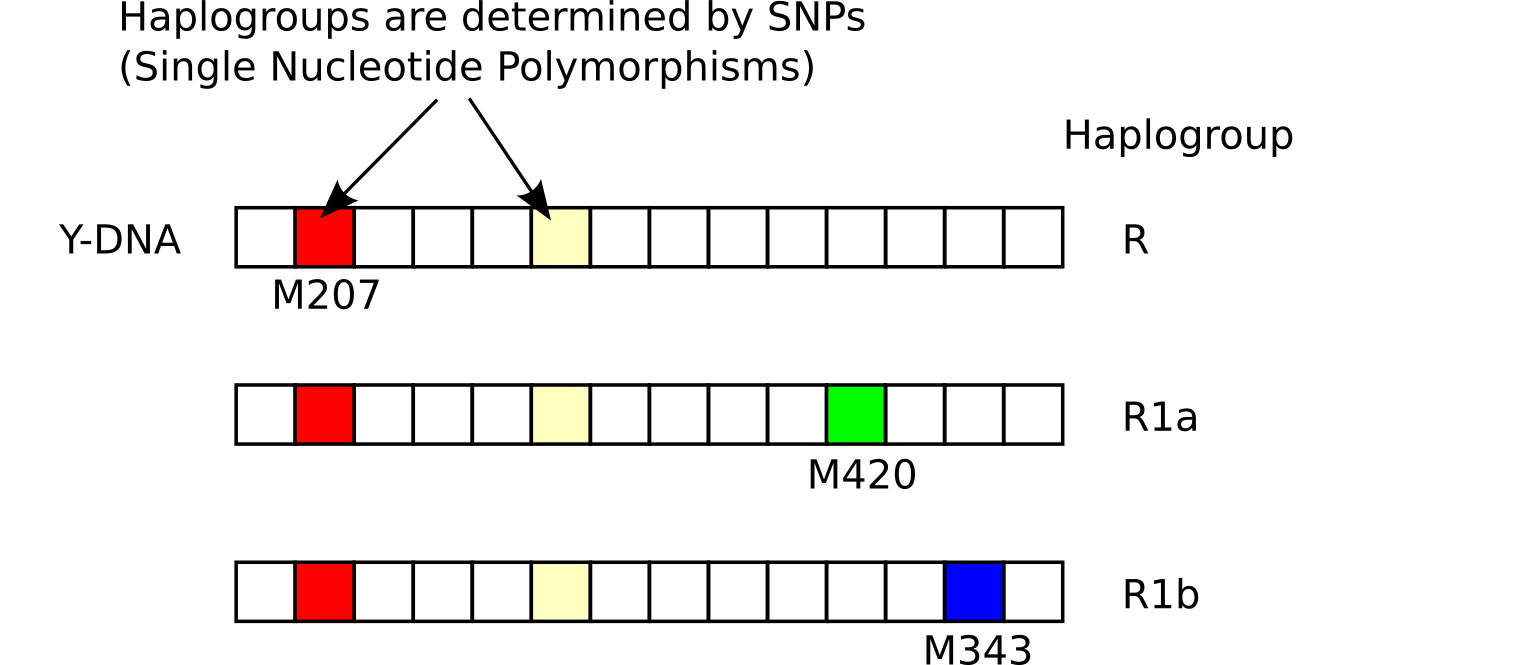
\includegraphics[width=13cm]{img/haplogroups.png}
\caption{\label{haplogroup} A set of single mutations
defines a person's haplogroup. Persons who belong to the
same haplogroup usually share a common ancestor within a
few thousand years.}
\end{figure}

Figure \ref{haplogroup} illustrates a typical situation.
Many Europeans belong to haplogroup R, which is characterized
by the mutation M207 and others which are not mentioned here.
The M207 marker is inherited throughout all following ancestral
lines. Later the mutations M420 and M343 occurred. They are
mutually exclusive to each other thus defining separate
lineages. The marker M420 defines the haplogroup R1a which
is common in Eastern Europe and the marker M343 defines the
haplogroup R1b which is common in Western Europe. Because
all people who belong to R1a and R1b share the M207 marker
we know that they also share a common ancestor a long time
ago.

SNPs do not occur very often. Persons who belong to the
same haplogroup usually share a common ancestor within a
few thousand years. If you know your haplogroup it will
tell you something about your deep history (thousands
of years).


\subsection{Haplotypes}

Most people want to know more about family relationships.
Luckily there is another type of mutations that occurs much
more often than SNPs. This is the repetition of certain
genetic patterns. They are called STRs (Short Tandem Repeats)
and group people into haplotypes.

\begin{figure}[ht]
\centering
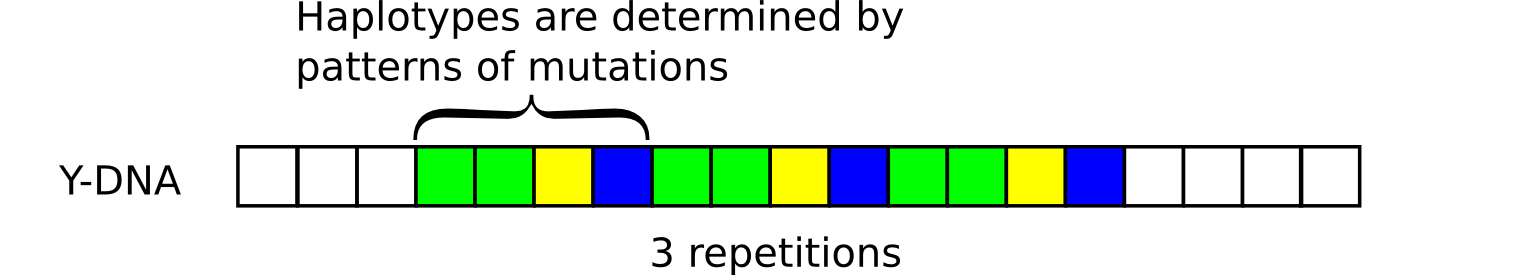
\includegraphics[width=13cm]{img/haplotypes.png}
\caption{\label{haplotype} A person's haplotype is defined
by patterns of mutations. Persons with the same haplotype
usually share a common ancestor within a few hundred years
if they take a standard test with 37 markers or more.}
\end{figure}

On the Y chromosome there are many different patterns that
repeat themselves. Every pattern has a name, for example DYS393.
If we count the number of repetitions for a specific pattern
we get a value, for example DYS393=13. Figure \ref{haplotype}
illustrates the situation for an exemplary marker. The pattern
is repeated 3 times. So this marker has a value of 3.

If a mutation occurs the number of repetitions changes. A 
single marker mutates rarely but the modern standard tests
use many markers at the same time, most often 37, 67 or
111. The combination of all these markers defines
a haplotype. Persons who share the same haplotype usually
also share a common ancestor within a few hundred years.

It is important to realize that haplotypes are not as good
as haplogroups. Haplotypes sometimes overlap between separate
lineages. So when working with haplotypes the haplogroup
should also be known.

Phylofriend uses haplotypes to calculate genetic distances
between persons by counting the number of different mutations.


\subsection{Phylogenetic Trees}

Phylogenetic trees group people together according to their
genetic distances. They give us a picture of how different
persons are related.

\begin{figure}[ht]
\centering
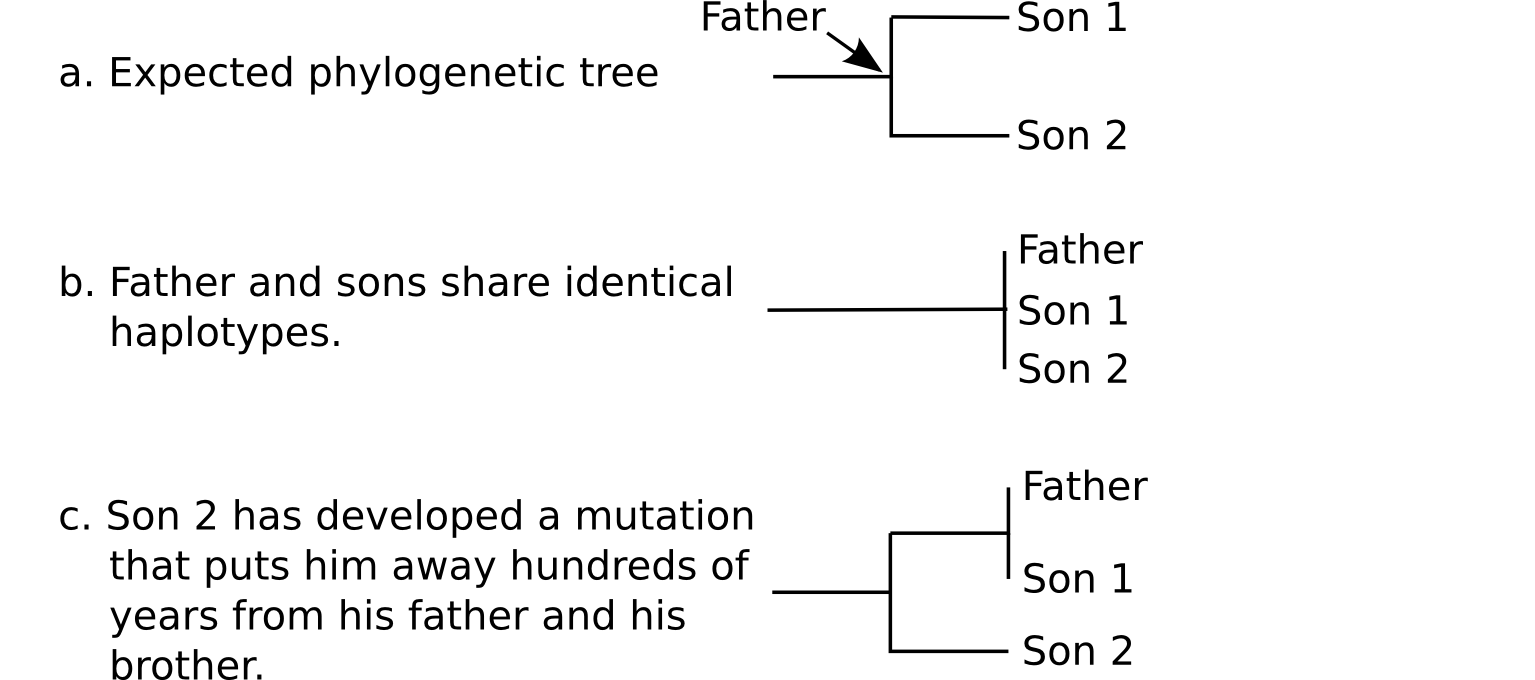
\includegraphics[width=13cm]{img/phylotrees.png}
\caption{\label{phylotrees} Phylogenetic trees group persons
together according to their genetic distances. Genetic
distances are often associated with time scales but this
is only true for long time spans.}
\end{figure}

Figure \ref{phylotrees} shows some exemplary trees. If a
father has two sons we would expect that both sons are at
a little genetic distance away from their father. If they
are not twins they also should be separated by each other.
Tree a illustrates this situation. This is exactly the
tree we would get if we could measure the genetic distance
at a high resolution and know the birth dates of father and
sons. Because we know the birth dates we would put the father
before the sons and associate the horizontal axis with a
time scale assuming that genetic distance is proportional
to time.

Reality however shows a different picture. The currently
available standard tests (37, 67 and 111 markers) only offer
a low resolution. So most often we can not measure any genetic
distance between father and sons. This is illustrated by
tree b. Because the tree illustrates genetic distances and
not time distances father and sons are all side by side.

If son 2 develops a mutation by chance we get a confusing picture.
Son 2 is suddenly far away from his father and his brother.
This is shown by tree c. The reason for the great distance
between father and son 2 is the low resolution of the test.
If we take the mutation rates from \cite{Kly12} we can
calculate how long it takes on average for a mutation to
occur. For a 37 marker test the result is 280 years, for
a 67 marker test 210 years and for a 111 marker test 130
years. 

This means if the father and his sons took a 37 marker test
and son 2 has developed a mutation by chance he will appear
to be 280 years away from his father but the only reason for
that is the low resolution of the test.

In most cases the standard tests are good enough. We do not
need a paternity test for genealogical purposes but it is
important to remember that the standard tests only places
persons into time frames of hundreds of years.


\subsection{Genetic Distance}

There are many ways to calculate genetic distances. Here we
use the method of mutation counting as described by Anatole
Klyosov in \cite{Kly09}.
We just count the number of mutation one persons differs from
another and take the result as the genetic distance.
Take a look at these two 6-marker haplotypes:

\vspace{1em}
\begin{tabular}{lrrrrrr}
       & DYS393 & DYS390      & DYS19 & DYS391      & DYS385a & DYS385b \\
Carl   &     13 & 24          & 14    & 11          & 11      & 14 \\
Clas   &     13 & \textbf{23} & 14    & \textbf{12} & 11      & 14
\end{tabular}
\vspace{1em}

At DYS390 and DYS391 Clas differs from Carl by one mutation.
Thus their genetic distance on the 6-marker scale is 2.

To represent this genetic distance in years we need to know
how often mutations occur. Thus we need a mutation rate.
The mutation rate is defined as follows:

\begin{equation}
k = \frac{m}{g Y} \label{mutationrate}
\end{equation}

\begin{tabular}{ll}
k: &  Mutation rate per marker and generation\\
m: &  Number of mutations \\
g: &  Number of generations \\
Y: &  Number of Y-STR values (markers)
\end{tabular}
\vspace{1em}

Mutation rates are derived from sample populations. Different
family lineages often expose different mutation rates. So the
standard mutation rates should be considered as a first 
estimate. You can uses Phylofriend's \emph{cal} option to
adjust your data to historic events.

Now we can use formula \ref{mutationrate} to calculate a
genetic distance in generations. Formula \ref{mutationrate}
is equivalent to:

\begin{equation}
g = \frac{m}{k Y} \label{generationdistance}
\end{equation}

This gives us the number of generations between Carl and Clas.
The only thing we still need to know is the generation time.
For historical purposes a generation time of 25 years is
commonly used. We get the time by multiplying the number
of generations with the generation time.

\begin{equation}
t = g d 
\end{equation}

\begin{tabular}{ll}
t: &  Genetic distance in years\\
g: &  Number of generations \\
d: &  Generation time in years
\end{tabular}
\vspace{1em}

By substituting $g$ with formula \ref{generationdistance}
we get the genetic distance in years:

\begin{equation}
t = \frac{m d}{k Y}
\end{equation}

\begin{tabular}{ll}
t: &  Genetic distance in years\\
m: &  Number of mutations \\
d: &  Generation time in years\\
k: &  Mutation rate per marker and generation\\
Y: &  Number of Y-STR values (markers)
\end{tabular}
\vspace{1em}

Let us try this out. The number of mutations between Clas
and Carl is 2. The mutation rate for a 6-marker haplotype
is 0.002 \cite{Kly09}. So

\begin{equation}
t = \frac{2 \cdot 25}{0.002 \cdot 6} = 4167 years
\end{equation}

Wow, that is a very long time. But what does this number
actually mean? First, it is an average value and there is
a very big margin of error to it but it is useful as a first
estimate and to group people together according to their
genetic distance. Second it is the time Clas and Carl would
be separated if Clas would be an ancestor of Carl (or the
other way round). It is not the time to their most recent
common ancestor (TMRCA).

If Clas and Carl would be living today, how long would be the
the time to their most recent common ancestor? The first guess
is that the common ancestor would be in-between his descendants
in terms of genetic distance. So Claus and Carl would be
$4167years / 2 = 2085years$ away from him. 

This is a good first guess but unfortunately reality is much
more complicated. Mutations occur by coincidence and due to
the laws of statistics some people develop only a few mutations
while others develop much of them. So our first guess may give
a totally wrong impression. Generally it is not a good idea to
calculate the time to a common ancestor just based on the results
of two people. The best way is to identify a group of people who
share a common lineage and calculate the time to the most recent
common ancestor for the whole group. Anatole Klyosov describes
how this is done in \cite{Kly09}.

For those who still want to use a TMRCA value based on the results
of just two people Bruce Walsh has developed a method to give
a time estimate\cite{Wal01}. This is better than the naive
calculation we have used before but it is still an estimate and
it is only valid for demographically stable populations.

The whole story is of course more complicated than the simple
calculation presented here. Different mutation models exist
and some genetic markers should be treated in a special way.
Phylofriend uses a hybrid mutation model that is a mixture
of the stepwise mutation model and the infinite alleles model.
Both models are explained by Bruce Walsh in \cite{Wal02}.


\subsection{From Distances to Trees}

Phylofriend computes genetic distances between different
persons. These distances can be used to derive phylogenetic
trees using standard algorithms that are implemented by
the PHYLIP\cite{Phylip} program.

Genetic distances are often represented by two-dimensional
drawings that are easy to understand. Here we label the
distance components as \emph{Component 1} and 
\emph{Component 2}. Usually the values for each component
are derived from many markers by using principal component
analysis\cite{Shl09}.

\begin{figure}[ht]
\centering
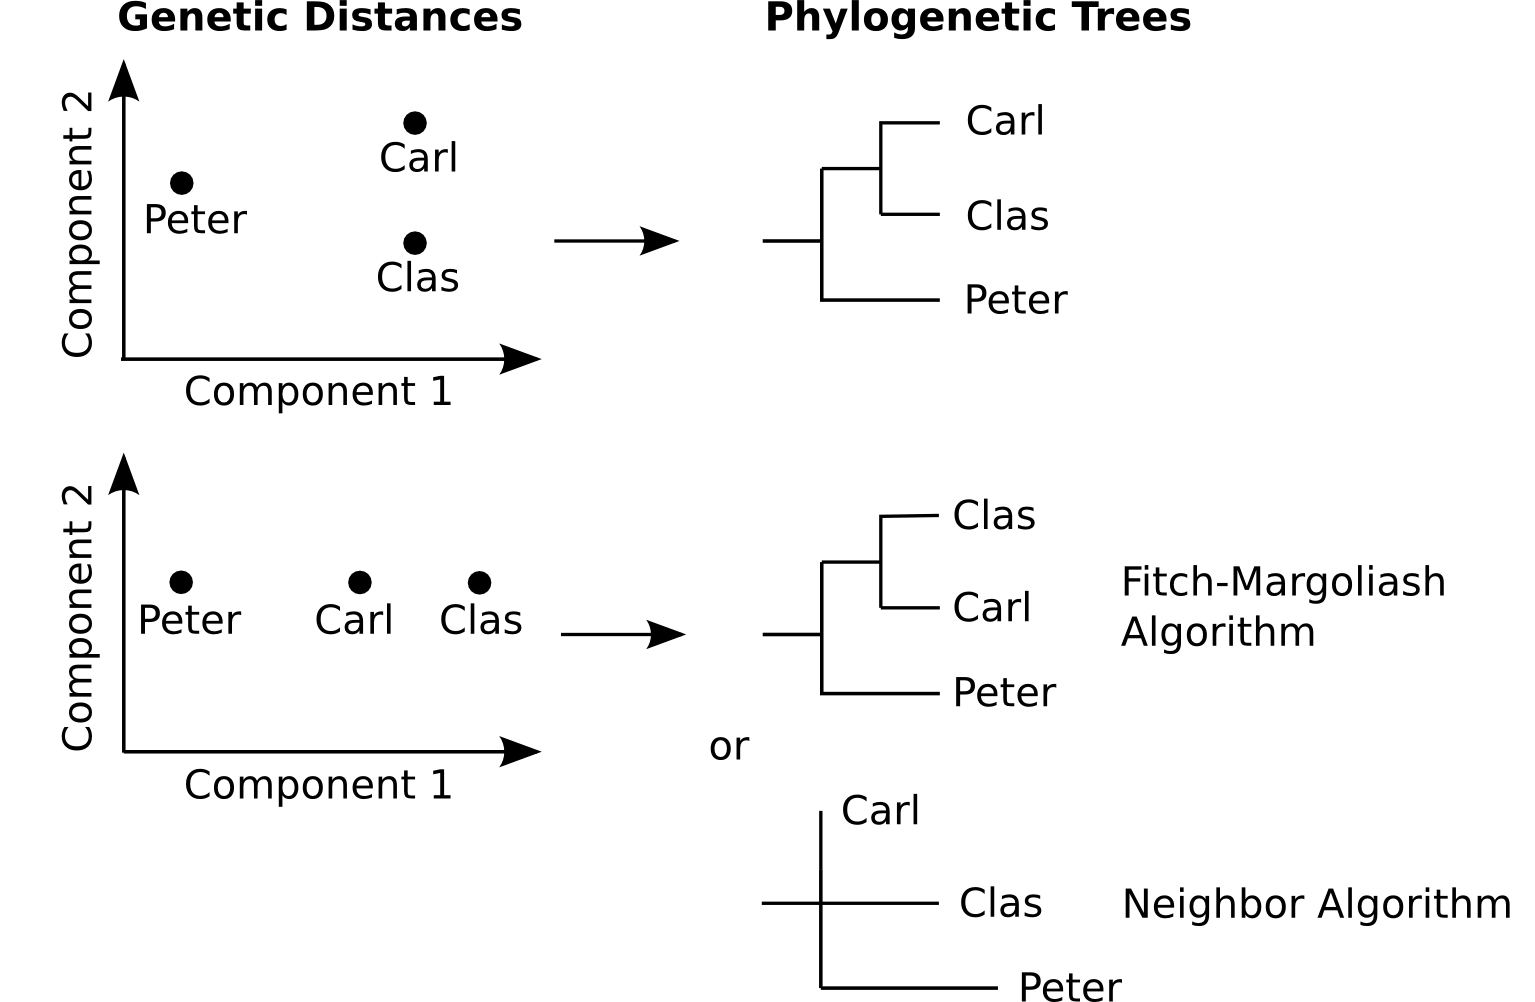
\includegraphics[width=13cm]{img/distancetrees.png}
\caption{\label{distancetrees} Genetic distances can be
represented by phylogenetic trees. Different algorithms
often yield different results.}
\end{figure}

Figure \ref{distancetrees} shows the genetic positions of
several persons and the corresponding phylogenetic trees.
In the first example Carl and Clas are close together. So
they are also grouped together in the tree. Peter is at a
longer distance but the distance to Carl and Clas is the
same. Thus he is put into a separate branch. The genetic
distance between the persons is represented by the length
of the horizontal lines in the tree.

The second example is slightly more complicated. Carl and
Clas are still close together but Peter is at a different
distance to each of them. The trees were constructed by
using two different methods, Fitch-Margoliash (kitch program)
and Neighbor. Fitch-Margoliash groups Carl and Clas together
and puts Peter at a medium distance from both of them. This
is a sensible approach because some people develop many
mutation and others develop less. So the ancestor of Carl and
Clas was probably somewere in-between. However the resulting
tree does not represent the genetic distances correctly but
it displays a very nice representation of temporal evolution.

The neighbor method tries to represent the genetic distances
as good as possible. In this case it is accurate but it gives
you a bad idea of temporal evolution.

For a high quality data set both methods should yield similar
results in grouping people together. The real problem is that
mutations occur by coincidence and we often have a very sparse
collection of descendants who are at large genetic distances
to each other.

\begin{figure}[ht]
\centering
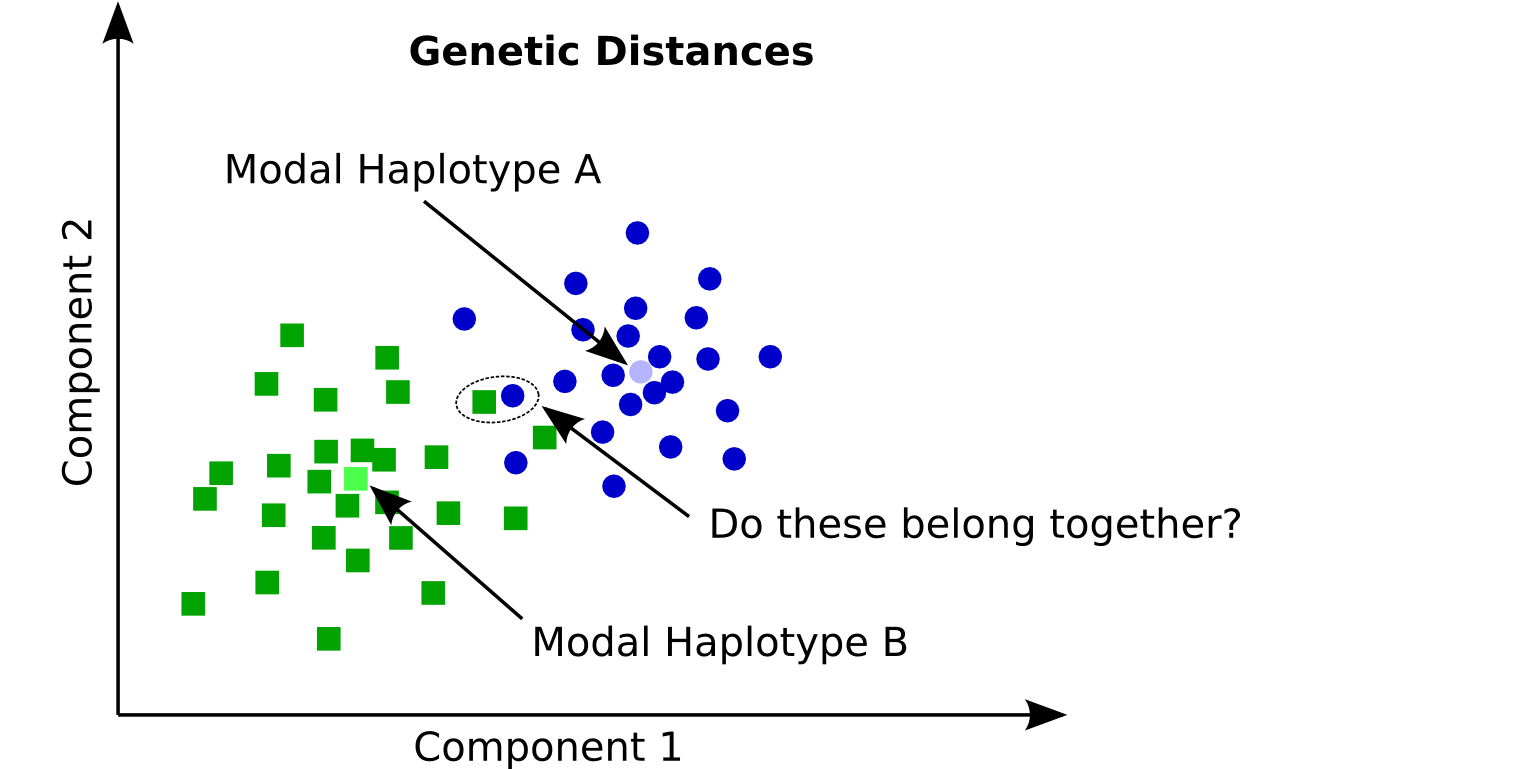
\includegraphics[width=13cm]{img/distances.png}
\caption{\label{distances} Haplotypes and genetic distances
of two families. Although both lineages have a different modal
(ancestral) haplotype the haplotypes of individuals from
both families are sometimes close together. In such cases
phylogenetic tree algorithms yield wrong results.}
\end{figure}

Figure \ref{distances} shows a more realistic situation.
It represents the genetic positions of members from two
different families. All members of one family descent from
one common ancestor. Due to the laws of statistics most
family members are close to his haplotype. So it can be
calculated. It is called the ancestral or modal haplotype.

Other family member are at a greater distance from the
ancestor. Sometimes members from different families come
close to each other. In such cases all algorithms will 
give you wrong results.

This is the reason why it is so important to test for
haplogroups before creating a phylogenetic tree. Haplogroups
are caused by very stable mutations. Haplotypes often overlap.
So it should be ensured that all persons in a tree belong
to the same haplogroup.





















\raggedright
\begin{thebibliography}{bla}

\bibitem{YFullMutationRate} Dmitry Adamov, Vladimir Guryanov,
Sergey Karzhavin, Vladimir Tagankin, Vadim Urasin.
\emph{\href{http://rjgg.molgen.org/index.php/RJGGRE/article/view/151}
{Defining a New Rate Constant for Y-Chromosome SNPs based on Full Sequencing Data}}.
The Russian Journal of Genetic Genealogy
(\foreignlanguage{russian}{Русская версия}),
Vol 6, No 2 (2014)/Vol 7, No 1 (2015).

\bibitem{Newick} James Archie, William H.E. Day, Wayne Maddison,
Christopher Meacham, F. James Rohlf, David Swofford, Joe Felsenstein,
\emph{\href{http://evolution.genetics.washington.edu/phylip/newicktree.html}
{The Newick Tree Format}}.
1986, Date accessed: 2014-08-06.

\bibitem{Trex} Alix Boc, Alpha Boubacar Diallo, Vladimir Makarenkov,
\emph{T-REX: a web server for inferring, validating and
visualizing phylogenetic trees and networks}.
Nucleic Acids Research (2012) 40 (W1): W573-W579.
\href{http://dx.doi.org/10.1093/nar/gks485}{doi: 10.1093/nar/gks485}, 2012. 

\bibitem{Can14} R. A. Canada,
\emph{\href{https://www.familytreedna.com/learn/y-dna-testing/y-str/infinite-allele-palindromic-markers/}
{How does the infinite allele comparison method work for palindromic markers?}}.
Family Tree DNA, 2014, Date accessed: 2014-08-07.

\bibitem{BigYWhitePaper} Family Tree DNA,
\emph{\href{https://www.familytreedna.com/learn/wp-content/uploads/2014/08/BIG_Y_WhitePager.pdf}{Big Y White Paper}}.
Family Tree DNA, August 2014.

\bibitem{Phylip} Joe Felsenstein,
\emph{\href{http://evolution.genetics.washington.edu/phylip.html}
{PHYLIP, a free package of programs for inferring phylogenies.}}.
University of Washington, First version: 1980, Date accessed: 2014-08-06.

\bibitem{Ham15} David Hamilton,
\emph{\href{http://biorxiv.org/content/early/2015/06/19/020933}
{An accurate genetic clock}},
bioRxiv preprint, first posted online June 15, 2015,
\href{http://dx.doi.org/10.1101/020933}{doi: 10.1101/020933}.

\bibitem{Kly09} Anatole A. Klyosov,
\emph{\href{http://www.jogg.info/52/files/Klyosov1.pdf}
{DNA Genealogy, Mutation Rates, and Some Historical
Evidence Written in Y-Chromosome, Part I:  Basic Principles and
the Method}}.
Journal of Genetic Genealogy, 5(2):186-216, 2009.

\bibitem{Kly12} Anatole A. Klyosov,
\emph{Ancient History of the Arbins, Bearers of Haplogroup R1b, from
Central Asia to Europe, 16,000 to 1500 Years before Present}.
Advances in Anthropology, Vol.2, No.2, 87-105,
\href{http://dx.doi.org/10.4236/aa.2012.22010}{doi:10.4236/aa.2012.22010}, 2012.

\bibitem{ISOGGSNPCriteria} ISOGG,
\emph{\href{http://www.isogg.org/tree/ISOGG_SNP_Requirements.html}
{Listing Criteria for SNP Inclusion into the ISOGG Y-DNA Haplogroup Tree - 2015}}.
Date visited: 2015-10-06.

\bibitem{Shl09} Jonathon Shlens,
\emph{\href{http://rieke-server.physiol.washington.edu/People/Fred/Classes/545/shlens-pca.pdf}
{A Tutorial on Principal Component Analysis}}.
Center for Neural Science, New York University,
New York City, 
Systems Neurobiology Laboratory, Salk Insitute for Biological Studies,
La Jolla, 2009.

\bibitem{Wiki-List_of_DYS_markers} Wikipedia,
\emph{\href{http://en.wikipedia.org/wiki/List_of_DYS_markers}
{List of Y-STR markers}}.
Date accessed: 2014-08-15.

\bibitem{Wal02} Bruce Walsh,
\emph{\href{http://nitro.biosci.arizona.edu/ftDNA/models.html}
{Details on the various assumptions used in computing TMRCA}}.
Family Tree DNA, 2002, Date accessed: 2014-08-07.

\bibitem{Wal01} Bruce Walsh,
\emph{\href{http://www.ncbi.nlm.nih.gov/pmc/articles/PMC1461668/}
{Estimating the Time to the Most Recent Common Ancestor for the
Y chromosome or Mitochondrial DNA for a Pair of Individuals}}.
Genetics Society of America, 2001.

\end{thebibliography}

\bibliography{references}
\addcontentsline{toc}{section}{References}
\end{document}
